\documentclass[12pt]{article}
\usepackage[margin=1in]{geometry}
\usepackage{float}
\usepackage{graphicx} 

\title{OMSV Report}
\author{Leonardo Cortés}
\date{January 2024}

\begin{document}

\maketitle

\section{Introduction}
In Argentina, approximately 4,000 people die in traffic accidents each year. Despite efforts to reduce traffic accidents in many jurisdictions, it remains the leading cause of violent deaths in the country. Reports from the National Criminal Information System (SNIC) of the Ministry of Security reveal 19,630 deaths in traffic accidents nationwide between 2018 and 2022. These figures translate to an average of 11 fatalities per day due to traffic accidents.

In 2022 alone, there were 3,828 fatal accidents. Experts suggest that the likelihood of someone dying in a traffic accident in Argentina is two to three times higher than in a criminal incident.

\section{Objectives}
\subsection{General Objective}
To analyze data provided by the Observatory of Mobility and Road Safety (OMSV) to identify patterns, trends, and factors associated with homicides in traffic accidents in Buenos Aires City during the period 2016-2021. Based on these findings, generate key information to enable local authorities to take effective measures to reduce the number of fatalities in these incidents.

\subsection{Specific Objectives}
\begin{itemize}
    \item \textbf{Identify Temporal Patterns:} Analyze the distribution of homicides in traffic accidents throughout the period 2016-2021 to identify potential seasonalities, monthly or yearly trends, and notable events that may influence the incidence of these incidents.
    
    \item \textbf{Characterize Accidents by Key Variables:} Break down data to understand the relationship between variables such as victim type, victim's age, geographical location, time of day, among others, with the occurrence of homicides in traffic accidents. This will identify possible areas of focus for preventive measures.
    
    \item \textbf{Analyze Victim and Perpetrator Profiles:} Examine the demographic characteristics of victims and, where possible, accused individuals involved in fatal accidents. This could include factors such as age, gender, role in the accident, among others, to gain a more comprehensive understanding of the most affected population groups.
    
    \item \textbf{Identify Critical Areas and Propose Intervention Measures:} Use geospatial data to map locations with a higher incidence of homicides in traffic accidents. Based on this information, propose specific intervention measures, such as improvements in signage, changes in road infrastructure, or the implementation of educational programs.
\end{itemize}

\section{Analysis}
To maintain organization and a better understanding of the supplied data, the analysis was conducted in three stages.

\subsection{Temporal Analysis}
After cleaning and processing the data, an analysis of time variables was performed to identify regularities and trends over time, revealing the following aspects:
\begin{itemize}
    \item Due to the abrupt change in the number of accidents in 2019 and 2020, likely due to Covid-19, finding a precise regularity in the accident rate per year is not possible.
    
    \item In the last months of the year, there is an observed pattern of increased accidents, especially in December.
    
    \item The impact of accidents in December is reflected in the number of accidents in the summer, with this season having 4\% more accidents on average than others.
    
    \item A relationship is found in the increase of accidents on weekends in the early morning hours.
\end{itemize}

A graphical summary of the analysis is presented below.

\begin{figure}[H]
  \centering
  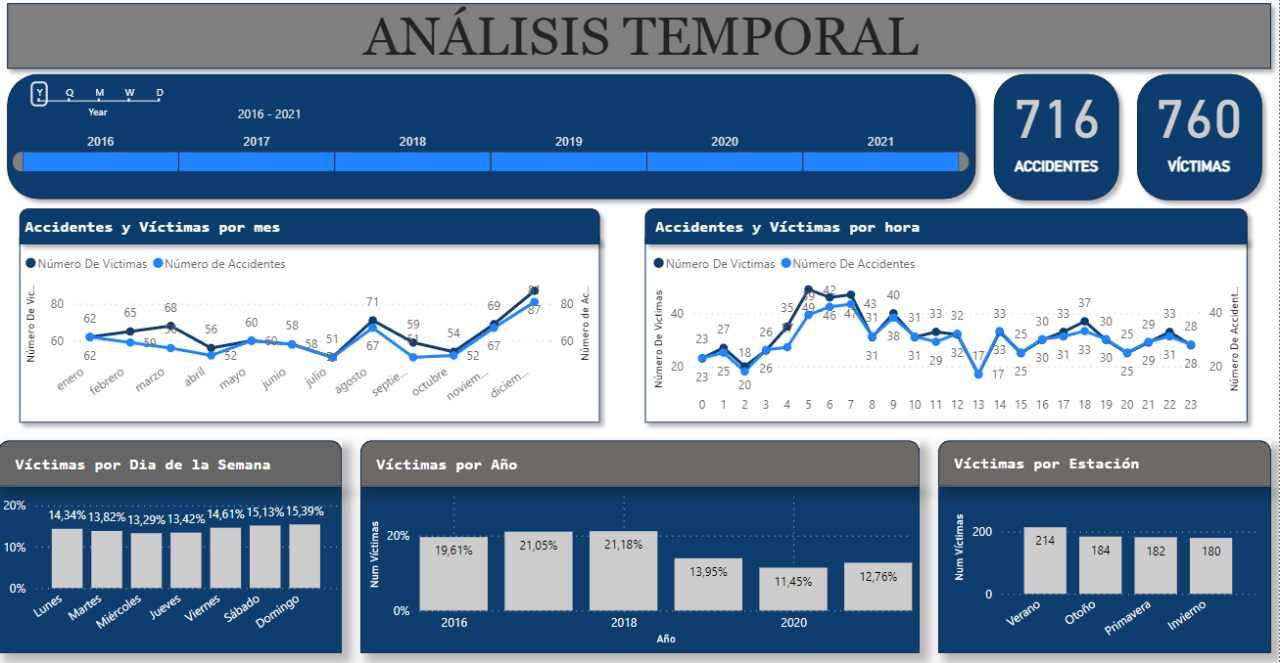
\includegraphics[width=0.8\textwidth]{Tem_Analysis.jpg}
  \caption{Temporal Analysis.}
  \label{fig:tem-analysis}
\end{figure}

\subsection{Geographical Analysis}
The analysis of the geographical situation of accidents in Buenos Aires City was also conducted based on the studied variables, revealing relevant information as follows:
\begin{itemize}
    \item The highest number of accidents occurs on avenues and primarily at intersections.
    
    \item With 98 accidents representing 13.6\% of the total accidents, Commune 1 has the highest number of accidents in the city.
    
    \item 51\% of accidents are concentrated in 5 out of the 15 communes (16 including boundaries).
    
    \item The Constitución neighborhood in Commune 1 records 36 accidents, approximately 37\% of the accidents in the commune with the highest accident rate. This is because it is also the commune with the most neighborhoods.
    
    \item The highest number of accidents accumulates to the east of the city.
\end{itemize}

A graphical summary of the analysis is presented below.

\begin{figure}[H]
  \centering
  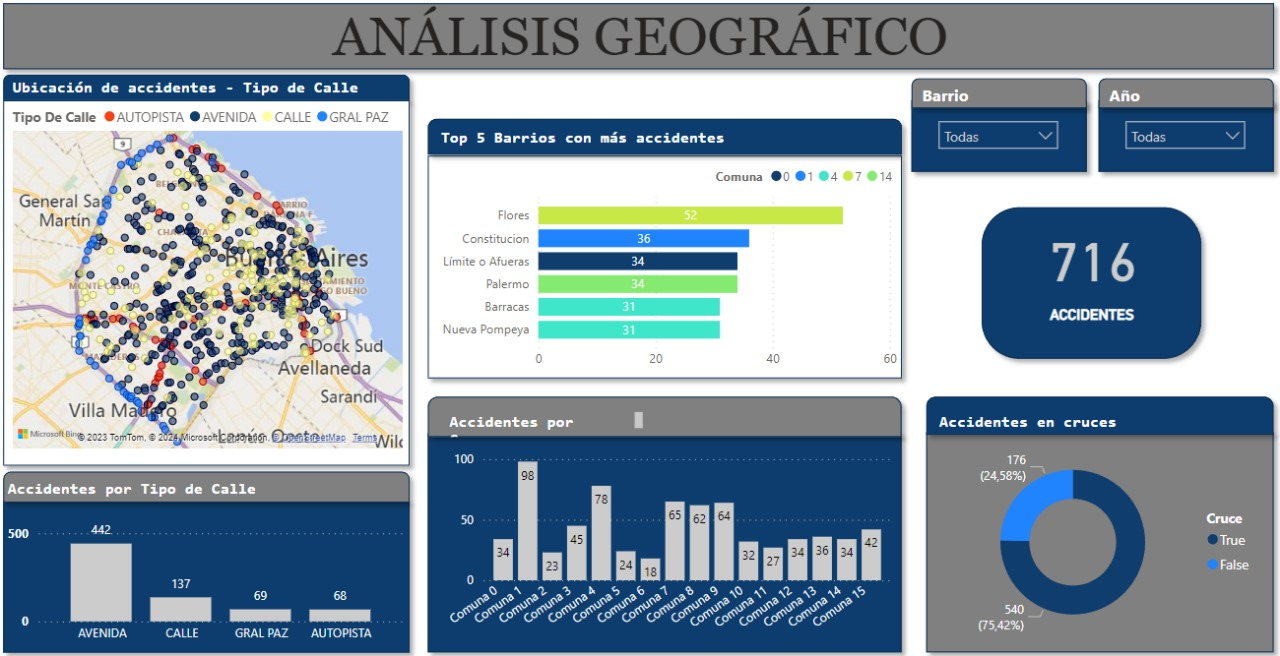
\includegraphics[width=0.8\textwidth]{Geo_Analysis.jpg}
  \caption{Geographical Analysis.}
  \label{fig:geo-analysis}
\end{figure}

\subsection{Victim Analysis}
An analysis of victims involved in traffic accidents was also conducted, examining patterns related to the role, age, gender, and vehicle of the individuals involved in accidents. From this analysis, the following conclusions were drawn:
\begin{itemize}
    \item Motorcyclists and pedestrians account for 589 victims, equivalent to 77\% of the total victims.
    
    \item The number of men involved in an accident is three times higher than the number of women.
    
    \item The majority of male victims are motorcyclists, while the majority of female victims are pedestrians.
    
    \item 47\% of victims were drivers, 35\% were pedestrians, and the remaining 18\% were distributed across different roles.
    
    \item The majority of victims are adults between 26 and 40 years old.
    
    \item Most female victims of traffic accidents are elderly individuals over 61 years old.
    
    \item The highest number of accidents was caused by automobiles.
\end{itemize}

A graphical summary of the analysis is presented below.

\begin{figure}[H]
  \centering
  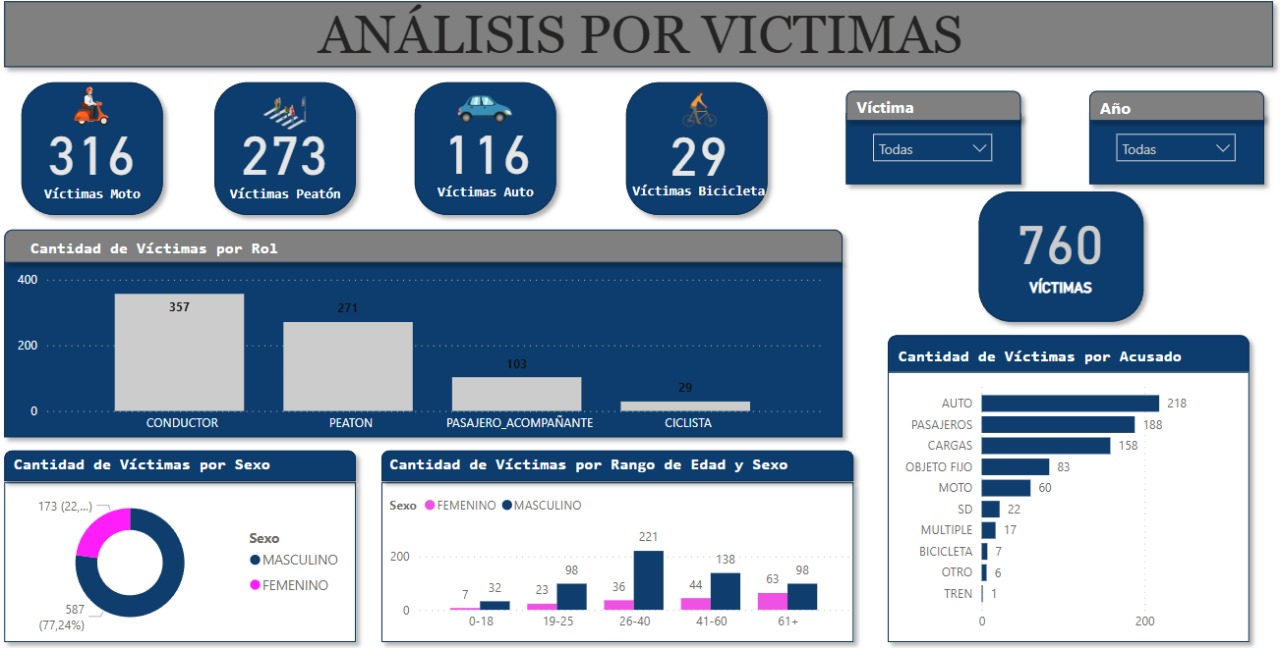
\includegraphics[width=0.8\textwidth]{Vic_Analysis.jpg}
  \caption{Victim Analysis.}
  \label{fig:vic-analysis}
\end{figure}

\subsection{Key Performance Indicators (KPIs)}
Three key performance indicators are proposed to assess progress in reducing accidents and make effective decisions to decrease the level of accidents in Buenos Aires City. The results of these indicators for the last evaluated period are shown below. However, final conclusions will be drawn regarding the overall analysis period, assessing the evolution of accidents.

\begin{itemize}
    \item \textbf{KPI 1:} Reduce the homicide rate in traffic accidents by 10\% in the last six months, in CABA, compared to the homicide rate in traffic accidents in the previous semester.

\begin{figure}[H]
  \centering
  \includegraphics[width=0.8\textwidth]{KPI1.png}
  \caption{KPI 1.}
  \label{fig:KPI 1}
\end{figure}

    This indicator shows that the goal is achieved for the last year, but there is no consistent pattern of fulfillment in previous years.

    \item \textbf{KPI 2:} Reduce the number of fatal accidents involving motorcyclists by 7\% in the last year, in CABA, compared to the previous year.

\begin{figure}[H]
  \centering
  \includegraphics[width=0.8\textwidth]{KPI2.png}
  \caption{KPI 2.}
  \label{fig:KPI 2}
\end{figure}

    In the last evaluated year, the indicator fails to meet its objective and significantly worsens, even though it had demonstrated an acceptable performance in previous years. This reveals a concerning trend for the most recent year.

    \item \textbf{KPI 3:} Reduce the number of fatal accidents caused by the driver (Accused Car) by 5\% in the last year.

\begin{figure}[H]
  \centering
  \includegraphics[width=0.8\textwidth]{KPI3.png}
  \caption{KPI 3.}
  \label{fig:KPI 3}
\end{figure}

    This indicator does not achieve its goal in the last evaluated year, and it has not achieved its goal in previous years. Therefore, closer attention to accidents evaluated by this indicator is recommended.
\end{itemize}

\section{Conclusions}
After proposing performance indicators related to the analysis and conclusions found in each of the three evaluated aspects, it is observed that the reduction in accidents has an unfavorable trend. The objectives are not consistently or precisely met in the specified time periods. Therefore, it is recommended to implement actions such as:

\begin{itemize}
    \item Traffic education campaigns.
    
    \item Raising awareness among the public about the social impact of traffic accidents.
    
    \item Stricter theoretical and practical tests for obtaining a driver's license.
    
\end{itemize}

These actions aim to achieve the objectives more consistently and regularly.
\\
\\
\\
\\
Without further ado, I am available for your comments, questions, and observations.
\\
\\
\\
\\

\section*{Signature}

Leonardo Cortés\\
Data Analyst \\
Date: January 2024

\end{document}
